\documentclass[../main.tex]{subfiles}
\addbibresource{../bibfile.bib}

\begin{document}

\chapter{Implementazione}
In questo capitolo, si fornirà una descrizione dettagliata dell'architettura della piattaforma Binoculars.
In particolare, verranno illustrare le implementazioni sia del frontend che del backend,
illustrando come la loro collaborazione permette all'utente di usare semplicemente le funzionalità offerte dalla piattaforma.
\section{Architettura}
L'architettura della piattaforma si suddivide in due componenti principali:
\begin{itemize}
    \item \textbf{Frontend}: Il frontend dell'applicazione comprende la logica di caricamento dei file binari e la presentazione
    dei risultati delle analisi. Questa componente è stata sviluppata utilizzando \textbf{SvelteKit}, un framework leggero e robusto per lo sviluppo
    di applicazioni web.
    \item \textbf{Backend}: Il backend dell'applicazione consiste in un server web sviluppato utilizzando il framework python \textbf{Flask}.
    In particolare, il server si occupa delle seguenti mansioni
    \begin{itemize}
        \item Gestione dei file binari caricati dall'utente
        \item Gestione della sessione HTTP
        \item Decompiling e Disassembly del file binario
        \item Applicazione delle diverse tecniche di analisi disponibili e generazione della risposta in formato \textit{JSON}
    \end{itemize}
\end{itemize}
\section{Backend}
Il server web è implementato in un singolo file \textit{wsgi.py} e utilizza il protocollo di trasmissione \textit{Web Server Gateway Interface} (WSGI)
per comunicare con il frontend.
In particolare, vengono esposti al frontend i seguenti endpoint:
\begin{itemize}
    \item \textbf{/upload}: Questo endpoint gestisce l'upload di file binari da parte degli utenti.
    Il file caricato deve essere un eseguibile \textit{ELF} valido; in caso affermativo, esso verrà memorizzato
    sulla piattaforma con un nome univoco. Questo meccanismo permette l'upload di file con nome uguale da parte
    di utenti diversi. Un'utente può caricare in piattaforma solamente un file alla volta.
    \item \textbf{/disassemble}: Questo endpoint gestisce l'attuazione del processo di disassembly sul file caricato.
    Questa operazione, come già esplicitato nel \textit{capitolo 4}, si sull'utilizzo della libreria python \textit{Capstone}.
    Alla termine del processo di disassembly, viene restituita una risposta HTTP contenete un file \textit{JSON} con la seguente struttura:
    \lstinputlisting[caption = Struttura del file JSON ritonrato dall'endpoint /disassemble]{../code_examples/disass_structure.json}
    \item \textbf{/decompile}: Questo endpoint gestisce il decompiling del file caricato tramite il framework \textit{Ghidra}.
    L'utilizzo da parte di \textit{Binoculars} di entrambi \textit{Ghidra} e \textit{angr} fa emergere un \textbf{conflitto sull'utilizzo dell'SMT solver \textit{Z3}}, il quale
    è utilizzato da entrambi i framework e non può essere utilizzato in un processo da più di un oggetto software alla volta.
    Per risolvere questo problema, il processo di decompilazione del file viene eseguito in un processo separato, il quale verrà terminato una volta completato
    il decompiling. Al termine dell'operazione, viene restituita una risposta HTTP contenente un file \textit{JSON} così strutturato:
    \lstinputlisting[caption = Struttura del file JSON ritonrato dall'endpoint /decompile]{../code_examples/decomp_structure.json}
    \item \textbf{/analyses/\{Analysis\}}: Questa famiglia di endpoint gestisce l'applicazione di una tecnica di analisi sul file eseguibile caricato.
    In particolare, \textit{Analysis} può assumere due possibili valori:
    \begin{itemize}
        \item \textbf{vulndetect}: Verrà applicata la strategia di analisi implementata da \textit{vulndetect}. Alla fine dell'analisi, verrà restituita una risposta
        HTTP contenente un file \textit{JSON} con la seguente struttura:
        \noindent
        \lstinputlisting[caption = Struttura del file JSON ritornato da vulndetect]{../code_examples/vulndetect_structure.json}
        \item \textbf{arbiter}: Verrà applicata la strategia di analisi implementata da \textit{Arbiter}. Alla fine dell'analisi, verrà restituita una risposta
        HTTP contenente un file \textit{JSON} con la seguente struttura:
        \lstinputlisting[caption = Struttura del file JSON ritonrato da arbiter]{../code_examples/arbiter_structure.json}
    \end{itemize}
\end{itemize}
Il codice del server web è riportato nell'\textit{appendice A} di questo documento.
\subsection{Configurazione}
Per garantite una più ampia flessibilità alla piattaforma, l'analista può configurare i seguenti parametri
del server web tramite un'apposito file \textit{JSON} di configurazione:
\begin{itemize}
    \item \textbf{Posizione cartella di upload}: Indica dove i file binari caricati dall'utente devono essere salvati.
    \item \textbf{Cartella di installazione di Ghidra}: In molte distribuzioni di Linux, \textit{Ghidra} è reperibile direttamente tramite il package manager della distribuzione.
    Questo parametro permette quindi all'analista di configurare correttamente la posizione di installazione del framework.
    \item \textbf{Massima profondità di angr}: Indica ad angr la massima profondità di esplorazione del CFG.
    \item \textbf{Cartella dei risultati di arbiter}: Indica dove i file JSON contenenti i risultati ottenuti da \textit{arbiter} devono essere salvati.
    \item \textbf{Cartella dei log di arbiter}: Indica dove i file di log di \textit{arbiter} devono essere salvati.
    \item \textbf{Cartella VD di arbiter}: Indica la posizione in cui si trovano i file contenenti le VD per \textit{arbiter}.
    \item \textbf{Regex per l'individuazione dei file VD}: Per permettere un recupero automatico dei file VD per arbiter, viene utilizzato un meccanismo di recupero basato su \textit{regex}.
    Questo parametro permette all'analista di configurare come i nomi dei file contenenti le VD per arbiter debbano essere formattati.
    \item \textbf{Blacklist di funzioni per arbiter}: Indica una lista di funzioni che \textit{arbiter} eviterà di analizzare.
\end{itemize}
\subsection{Implementazione delle tecniche di analisi}
Le due tecniche di analisi disponibili (\textit{Arbiter} e \textit{VulnDetect}) sono integrate nella piattaforma
attraverso l'utilizzo di due \textbf{classi wrapper}. Queste classi sono state \textbf{progettate} per offrire un
punto di accesso semplificato ad entrambe le metodologia. In particolare per \textit{Arbiter}, il quale utilizzo prevede un'esecuzione
tramite linea di comando, questa scelta è stata essenziale per semplificare l'accesso e l'attivazione della strategia di analisi da parte della piattaforma.
Il codice delle due classi wrapper è riportano nell'\textit{appendice A} di questo documento.
\section{Frontend}
Il frontend della piattaforma consiste in due pagine sviluppate tramite il framework \textit{Svelte}:
\begin{itemize}
    \item \textbf{Pagina principale}: La pagina principale dell'applicazione. Essa permette all'utente di caricare un file binario tramite un apposito pulsante di upload.
    \item \textbf{Pagina di analisi}: Questa pagina è dedicata all'analisi del file binario caricato dall'utente. Essa mostra i risultati del disassembly e del decompiling
    del programma e permette all'utente di lanciare una della analisi presenti sulla piattaforma e di ottenerne i risultati.
\end{itemize}
Inoltre, le due pagine condividono una \textbf{navbar}, la quale è stata sviluppata come componente indipendente, in modo che essa possa essere riutilizzata facilmente.
Il \textit{routing} tra la pagina principale e la pagina di analisi è gestito direttamente da Svelte attraverso il suo meccanismo di filesystem-based routing, 
il quale definisce le route dell'applicazione in base alla posizione dei file nelle directory del progetto. Questo meccanismo è stato utilizzato anche per implementare un \textbf{proxy},
così da poter effettuare le chiamate necessarie al backend dell'applicazione senza la necessità di dover configurare manualmente le politiche \textit{CORS} (\textit{Cross-Origin Resource Sharing}) per ogni chiamata. 
Gli endpoint esposti dal \textit{proxy} sono:
\begin{itemize}
    \item \textbf{/api/upload}: Effettua una chiamata all'endpoint \textit{/upload}.
    \item \textbf{/api/disassemble}: Effettua una chiamata all'endpoint \textit{/disassembly}.
    \item \textbf{/api/decompile}: Effettua una chiamata all'endpoint \textit{/decompile}.
    \item \textbf{/api/analyses/\{Analysis\}}: Effettua una chiamata all'endpoint \textit{/analyses/\{Analysis\}}, dove \textit{Analysis} può essere \textit{vulndetect} oppure \textit{arbiter}.
\end{itemize}
\subsection{Pagina principale}
La pagina principale dell'applicazione è la prima pagina che appare all'utente. Essa presenta in fondo una descrizione delle funzionalità della piattaforma (raggiungibile anche utilizzando il tasto \textit{about} della navbar)
e un pulsante, il quale permette all'utente di caricare un file eseguibile \textit{ELF} in piattaforma. In particolare, effettuare il caricamento di un file binario genera una chiamata all'endpoint \textit{/api/upload}, il quale, a sua volta
effettuerà una chiamata all'endpoint \textit{/upload} del backend. Se il caricamento del file ha successo (il file che l'utente sta cercando di caricare è un file \textit{ELF} valido), allora l'utente verrà reindirizzato alla pagina
di analisi del binario. Altrimenti, verrà mostrato un messaggio di errore all'utente, informandolo che il caricamento del file non è andato a buon fine.
\begin{figure}[H]
    \centering
    
\includegraphics[width = \textwidth]{../images/main page.png}
    \caption{Pagina principale dell'applicazione}
\end{figure}
\lstinputlisting[language = JavaScript, caption = Proxy per l'operazione di caricamento di un file]{../code_examples/main_page_proxy.js}
\subsection{Pagina di analisi}
La pagina di analisi è divisa in tre sezioni:
\begin{itemize}
    \item \textbf{Disassembled code}: Questa sezione contiene  il codice assembly ottenuto dal processo di disassembly del binario.
    \item \textbf{Decompiled code}: Questa sezione contiene il codice \textit{C-Like} ottenuto dal processo di decompiling tramite \textit{Ghidra}.
    \item \textbf{Vulnerability analyses}: Questa sezione presenta una maschera per la selezione della strategia di analisi da applicare.
    Dopo la selezione, la maschera mostra gli eventuali \textbf{parametri di input} che l'utente deve fornire prima di avviare l'analisi.
\end{itemize}
Quando la pagina viene caricata, vengono effettuate immediatamente due chiamate a \textit{/api/disassembly} e \textit{/api/decompile} per ottenere rispettivamente il \textit{disassembly} e il codice \textit{decompilato}
del programma. Qualora una di queste due chiamate non vada a buon fine, verrà visualizzato un messaggio di errore all'utente nella sezione associata alla chiamata fallita.
Altrimenti, verrà mostrato, nella sezione associata alla chiamata, il codice ottenuto.
Infine, l'utilizzo, da parte dell'utente, di una qualsiasi delle tecniche di analisi disponibili genera una chiamata a \textit{/api/\{Analysis\}}. Se la chiamata ha successo, al termine dell'analisi
verranno presentati i risultati ottenuti all'utente. Altrimenti, verrà mostrato un messaggio di errore.
\begin{figure}[H]
    \centering
    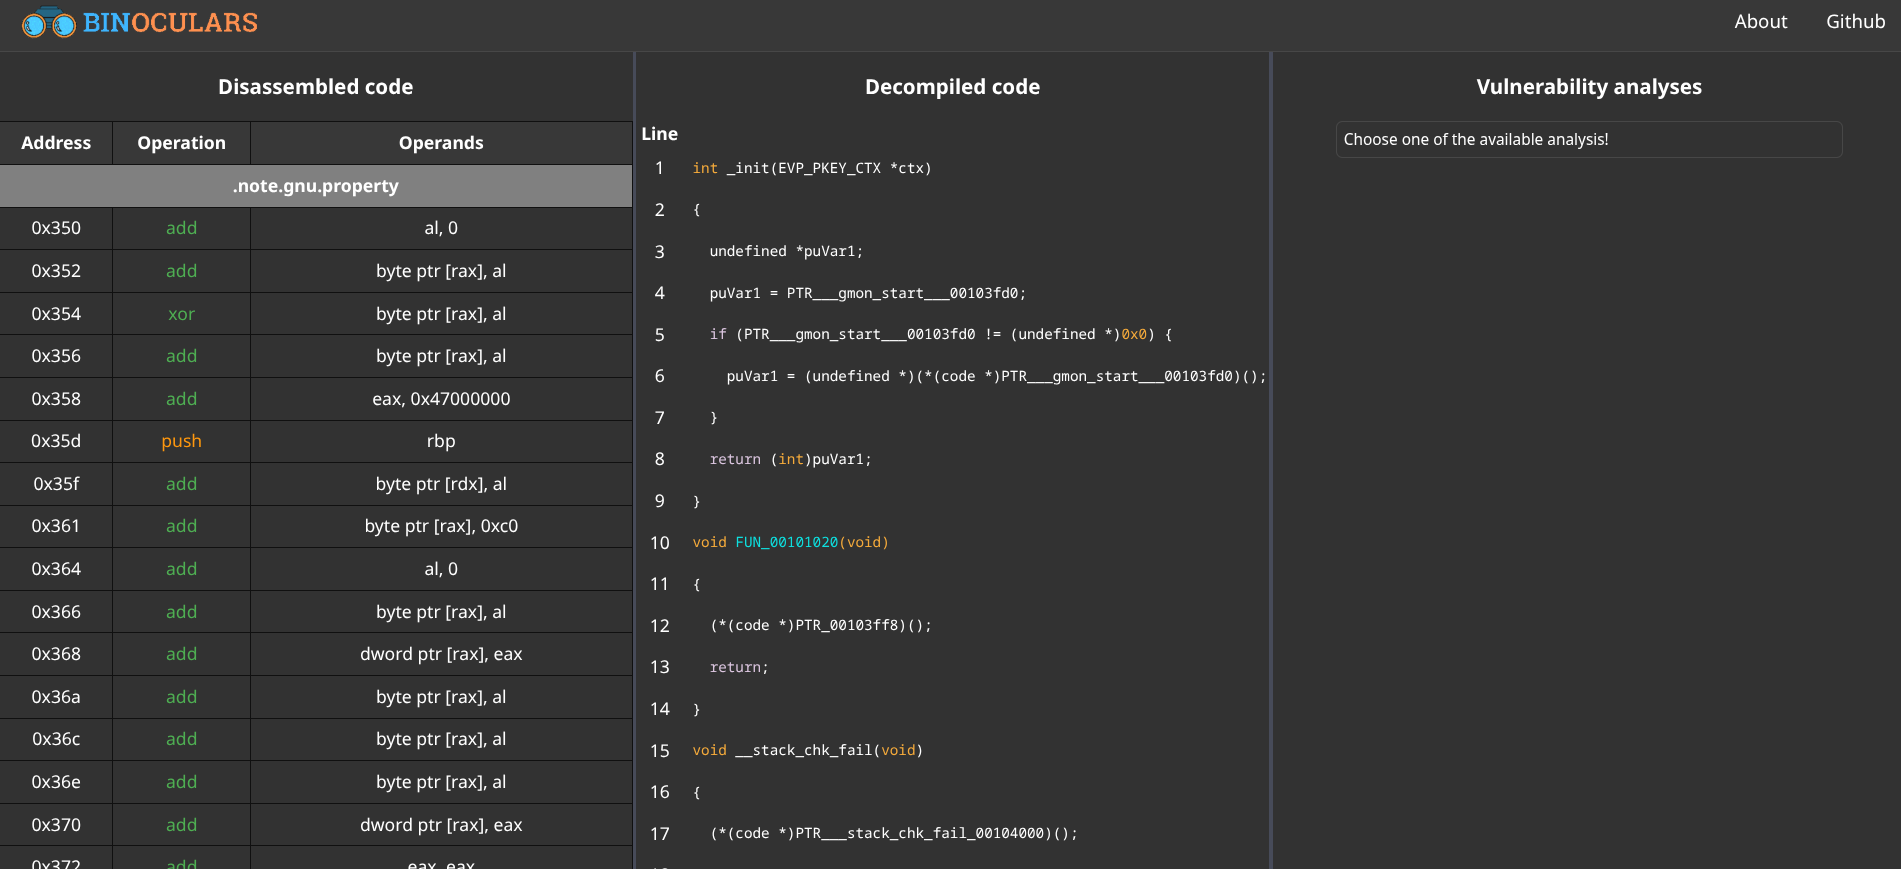
\includegraphics[width = \textwidth]{../images/analysis_page_no_results.png}
    \caption{Pagina di analisi dell'applicazione senza alcun risultato}
\end{figure}
\begin{figure}[H]
    \centering
    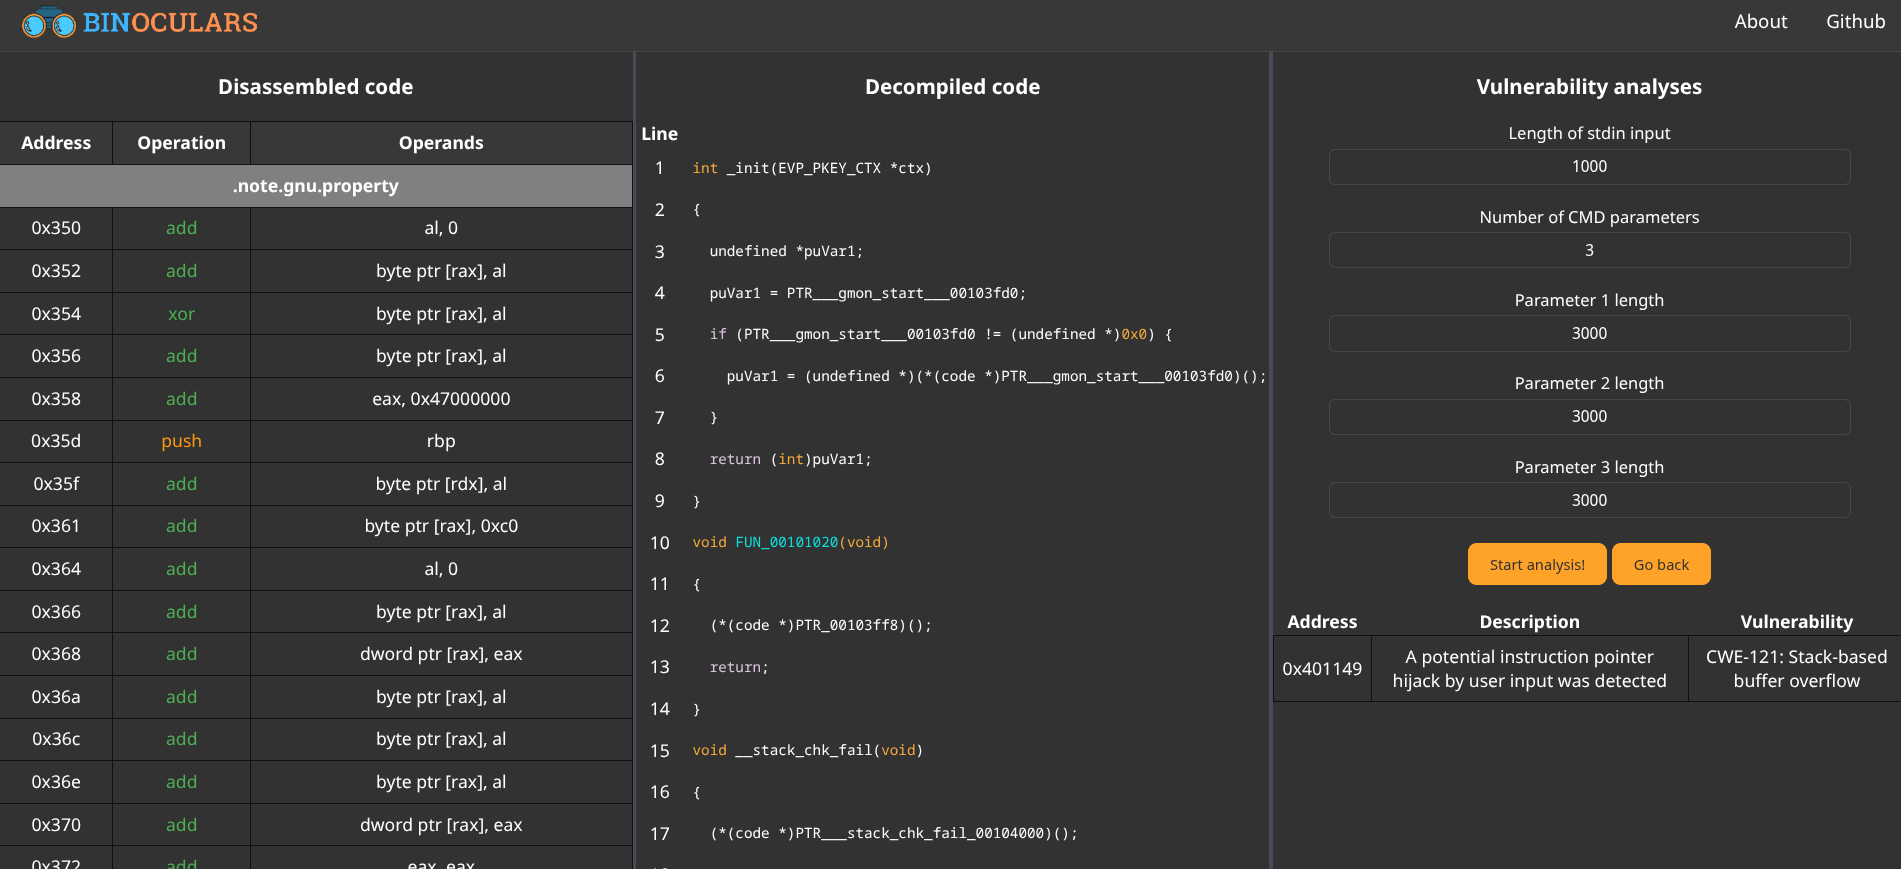
\includegraphics[width = \textwidth]{../images/analysis_page_vulndetect.png}
    \caption{Pagina di analisi dell'applicazione con i risultati ottenuti da \textit{VulnDetect}}
\end{figure}
\begin{figure}[H]
    \centering
    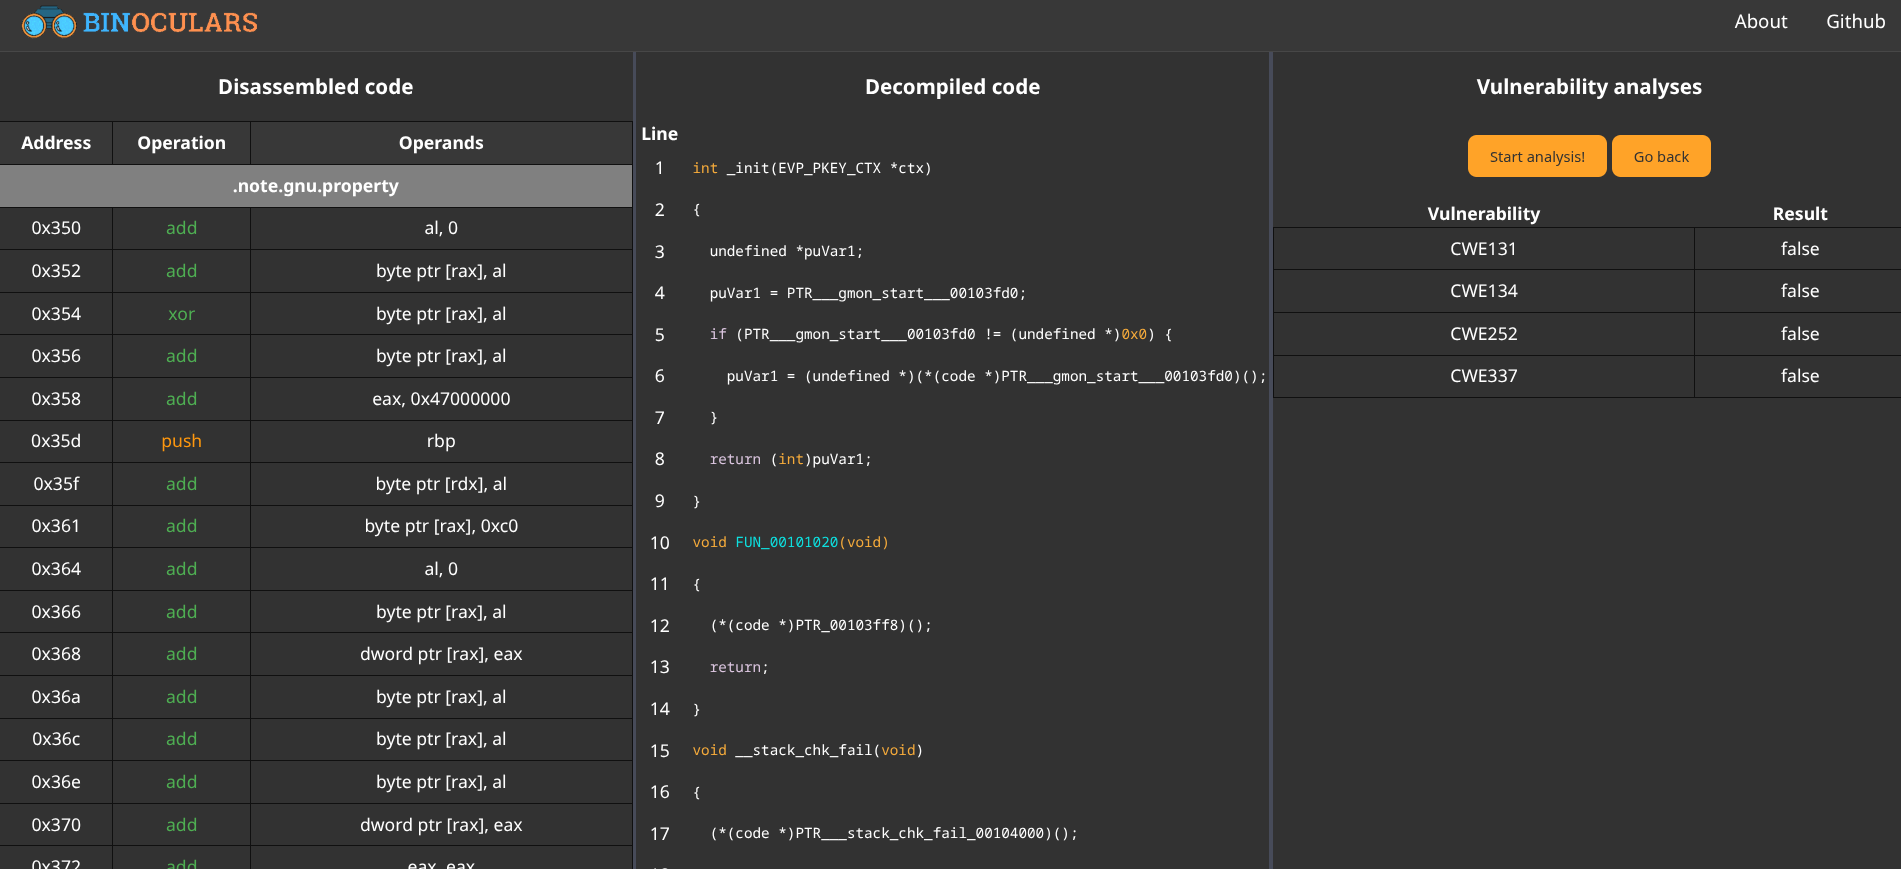
\includegraphics[width = \textwidth]{../images/analysis_page_arbiter.png}
    \caption{Pagina di analisi dell'applicazione con i risultati ottenuti da \textit{Arbiter}}
\end{figure}
\lstinputlisting[language = JavaScript, caption = Struttura di un proxy per le operazioni di analisi. \protect{\textit{Analysis}} può assumere il valore \protect{\textit{vulndetect}} oppure \protect{\textit{arbiter}}]{../code_examples/analysis_proxy.js}
\lstinputlisting[language = JavaScript, caption = Struttura di un proxy per le operazioni di disassembly e decompiling. \protect{\textit{Operation}} può assumere il valore \protect{\textit{disassemble}} oppure \protect{\textit{decompile}}]{../code_examples/disass_proxy.js}
\newpage
\lstinputlisting[language = JavaScript, caption = Funzione \textit{sendData} utilizzata dal codice riportato nel listing 6.9]{../code_examples/sendData.js}
\lstinputlisting[language = JavaScript, caption = Codice che svolge il recupero del disassembly e del decompiling tramite l'interrogazione del backend. Questo codice viene eseguito immediatamente dopo il caricamento della pagina di analisi]{../code_examples/fetch_code.js}
\end{document}